\documentclass[a4paper,12pt]{ctexart}

\usepackage{listings}
\usepackage{indentfirst}
\usepackage{xcolor}
\usepackage[colorlinks,linkcolor=black]{hyperref}
\usepackage{graphicx}
\usepackage{geometry}
\geometry{top=2.5cm,bottom=3.0cm,left=2.0cm,right=2.0cm}
\lstset{
	columns=fixed,
	numbers=left,
	breaklines=true,
	frame=shadowbox,
	commentstyle=\color{gray},
	rulesepcolor= \color{gray},
	numberstyle= \small,
	keywordstyle= \color{red},
	stringstyle=\rmfamily\slshape\color[RGB]{128,0,0},
	showstringspaces=false, 
	morekeywords={my,asm},
	showtabs=false,
	tabsize=4,
	title=\lstname,
	basicstyle=\ttfamily
}

\title{Android中的MVC}
\author{Will Also}
\date{2019}

\begin{document}
	\maketitle
	\tableofcontents
	\section{MVC}
	\subsection{MVC来源}
	MVC模式(Model–view–controller)是软件工程中的一种软件架构模式,把软件系统分为三个基本部分:模型(Model)、视图(View)和控制器(Controller)。
	\par MVC模式最早由Trygve Reenskaug在1978年提出,是施乐帕罗奥多研究中心(Xerox PARC)在20世纪80年代为程序语言Smalltalk发明的一种软件架构。MVC模式的目的是实现一种动态的程序设计,使后续对程序的修改和扩展简化,并且使程序某一部分的重复利用成为可能。除此之外,此模式透过对复杂度的简化,使程序结构更加直观。软件系统透过对自身基本部分分离的同时也赋予了各个基本部分应有的功能。
	\subsection{组件}
	\begin{itemize}
		\item 模型(Model) 用于封装与应用程序的业务逻辑相关的数据以及对数据的处理方法。
		 “Model”有对数据直接访问的权力,例如对数据库的访问。“Model”不依赖“View”和“Controller”,也就是说, Model 不关心它会被如何显示或是如何被操作。但是 Model 中数据的变化一般会通过一种刷新机制被公布(观察者模式)。
		 \item 视图(View)能够实现数据有目的的显示。在 View 中一般没有程序上的逻辑。为了实现 View 上的刷新功能,View 需要访问它监视的数据模型(Model),因此应该事先在被它监视的数据那里注册。
		 \item 控制器(Controller)起到不同层面间的组织作用,用于控制应用程序的流程。它处理事件并作出响应。“事件”包括用户的行为和数据 Model 上的改变。
	\end{itemize}
	\begin{figure}[ht]
		\centering
		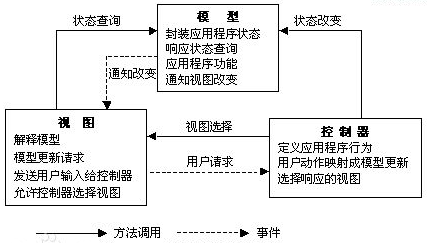
\includegraphics[]{image/1.png}
		\caption{MVC组件和行为}
	\end{figure}
	\subsection{优点}
	\begin{itemize}
		\item 耦合性低:视图层和业务层分离,这样就允许更改视图层代码而不用重新编译模型和控制器代码,同样,一个应用的业务流程或者业务规则的改变只需要改动MVC的模型层即可。
		\item 重用性高:MVC模式允许使用各种不同样式的视图来访问同一个服务器端的代码,因为多个视图能共享一个模型,它包括任何WEB(HTTP)浏览器或者无线浏览器(wap),由于模型返回的数据没有进行格式化,所以同样的构件能被不同的界面使用。
		\item 生命周期成本低:MVC使开发和维护用户接口的技术含量降低。
		\item 部署快:使用MVC模式使开发时间得到相当大的缩减,它使程序员(Java开发人员)集中精力于业务逻辑,界面程序员(HTML和JSP开发人员)集中精力于表现形式上。
		\item 可维护性高:分离视图层和业务逻辑层也使得WEB应用更易于维护和修改。Controller 提高了应用程序的灵活性和可配置性。
		\item 有利于软件工程化管理:由于不同的层各司其职,每一层不同的应用具有某些相同的特征,有利于通过工程化、工具化管理程序代码。
	\end{itemize}
	\subsection{缺点}
	\begin{itemize}
		\item 没有明确的定义:使用MVC需要精心的计划,由于它的内部原理比较复杂,模型和视图要严格的分离,这样也给调试应用程序带来了一定的困难。每个构件在使用之前都需要经过彻底的测试。
		\item 不适合小型,中等规模的应用程序,增加系统结构和实现的复杂性:对于简单的界面,严格遵循MVC,使模型、视图与控制器分离,会增加结构的复杂性,并可能产生过多的更新操作,降低运行效率。
		\item 视图与控制器间的过于紧密的连接:视图与控制器是相互分离,但却是联系紧密的部件,。
		\item 视图对模型数据的低效率访问:依据模型操作接口的不同,视图可能需要多次调用才能获得足够的显示数据。对未变化数据的不必要的频繁访问,也将损害操作性能。
		\item 一般高级的界面工具或构造器不支持模式:改造这些工具以适应MVC需要和建立分离的部件的代价是很高的,会造成MVC使用的困难。
	\end{itemize}
	\subsection{实现}
	\subsubsection{Java}
	\begin{itemize}
		\item 视图(View)可能由Java Server Page(JSP)担任。生成 View 的代码则可能是一个servlet的一部分,特别是在客户端服务端交互的时候。
		\item Controller 可能是一个servlet。
		\item Model 则是由一个实体Bean来实现。
	\end{itemize}
	\subsubsection{JavaScript}
	\begin{lstlisting}[morekeywords={var,data,render,handleOnload,onload}]
var M = {}, V = {}, C = {};
//Model
M.data = "hello world";
//View
V.render = (M) => { alert(M.data); }
//Controller
C.handleOnload = () => { V.render(M); }
window.onload = C.handleOnload;
	\end{lstlisting}
	\section{Android中的MVC}
	\subsection{MVC class}
	In a world where the user interface logic tends to change more often than the business logic, the desktop and Web developers needed a way of separating user interface functionality. 
	\begin{figure}[ht]
		\centering
		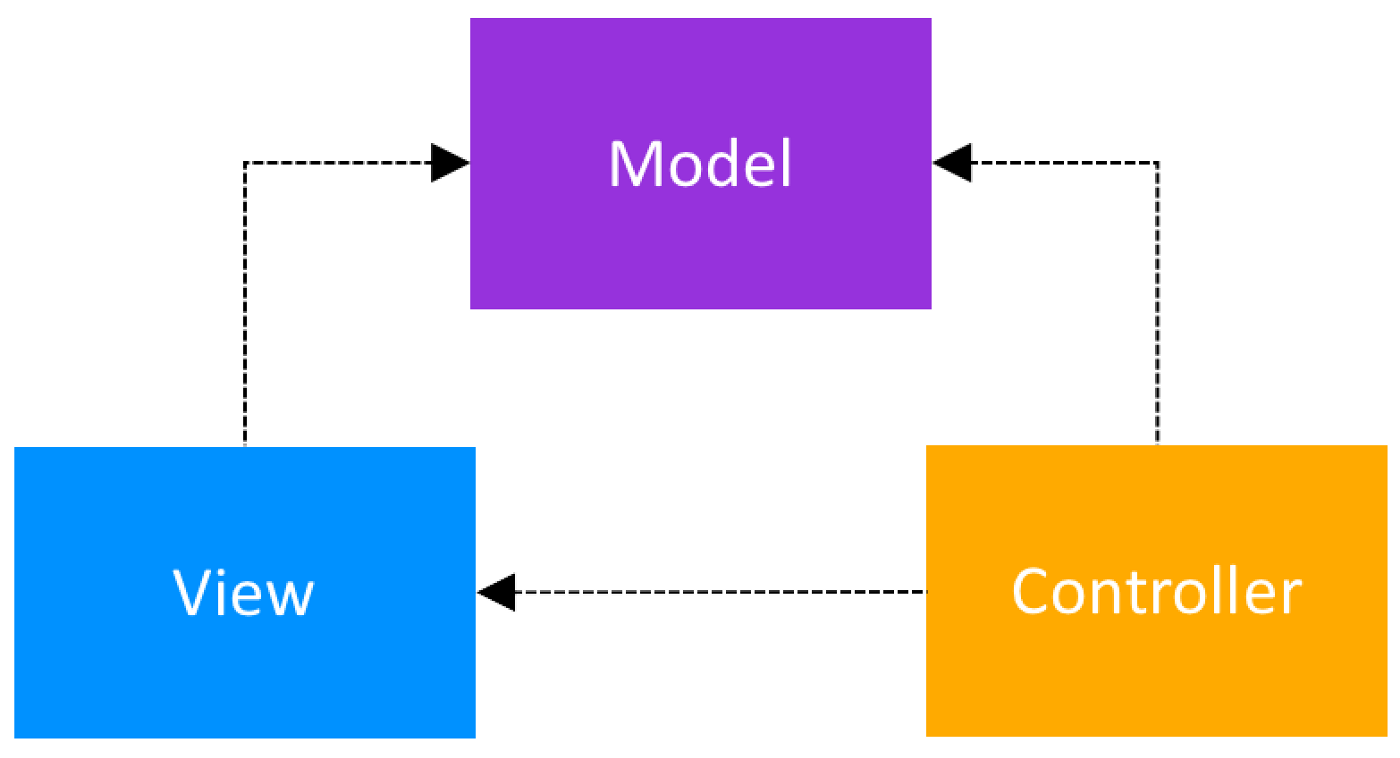
\includegraphics[width=\textwidth]{image/2.png}
		\caption{Model-View-Controller class structure}
	\end{figure}
	\subsection{MVC变体}
	This(Figure 2) means that both the Controller and the View depend on the Model: the Controller to update the data, the View to get the data. But, most important for the desktop and Web devs at that time: the Model was separated and could be tested independently of the UI. Several variants of MVC appeared. The best-known ones are related to whether the Model is passive or is actively notifying that it has changed.
	\subsubsection{Passive Model}
	In the Passive Model version, the Controller is the only class that manipulates the Model. Based on the user’s actions, the Controller has to modify the Model. After the Model has been updated, the Controller will notify the View that it also needs to update. At that point, the View will request the data from the Model.
	\begin{figure}[ht]
		\centering
		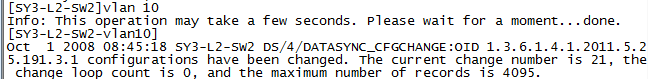
\includegraphics[width=\textwidth]{image/3.png}
		\caption{Model-View-Controller — passive Model — behavior}
	\end{figure}
	\subsubsection{Active Model}
	For the cases when the Controller is not the only class that modifies the Model, the Model needs a way to notify the View, and other classes, about updates. This is achieved with the help of \textbf{the Observer pattern}. The Model contains a collection of observers that are interested in updates. The View implements the observer interface and registers as an observer to the Model.
	\begin{figure}[ht]
		\centering
		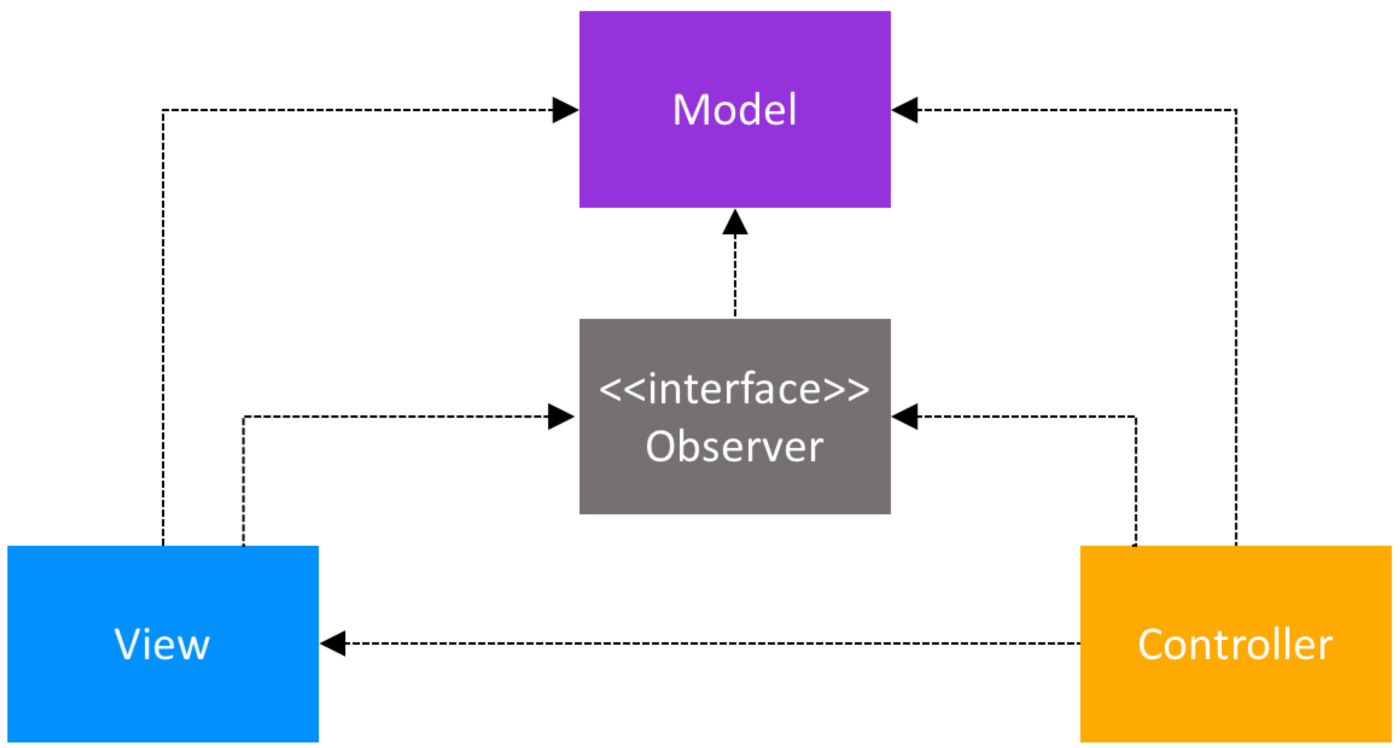
\includegraphics[width=\textwidth]{image/4.png}
		\caption{Model-View-Controller — active Model — class structure}
	\end{figure}
	Every time the Model updates, it will also iterate through the collection of observers and call the update method. The implementation of this method in the View will then trigger the request of the latest data from the Model.
	\begin{figure}[!h]
		\centering
		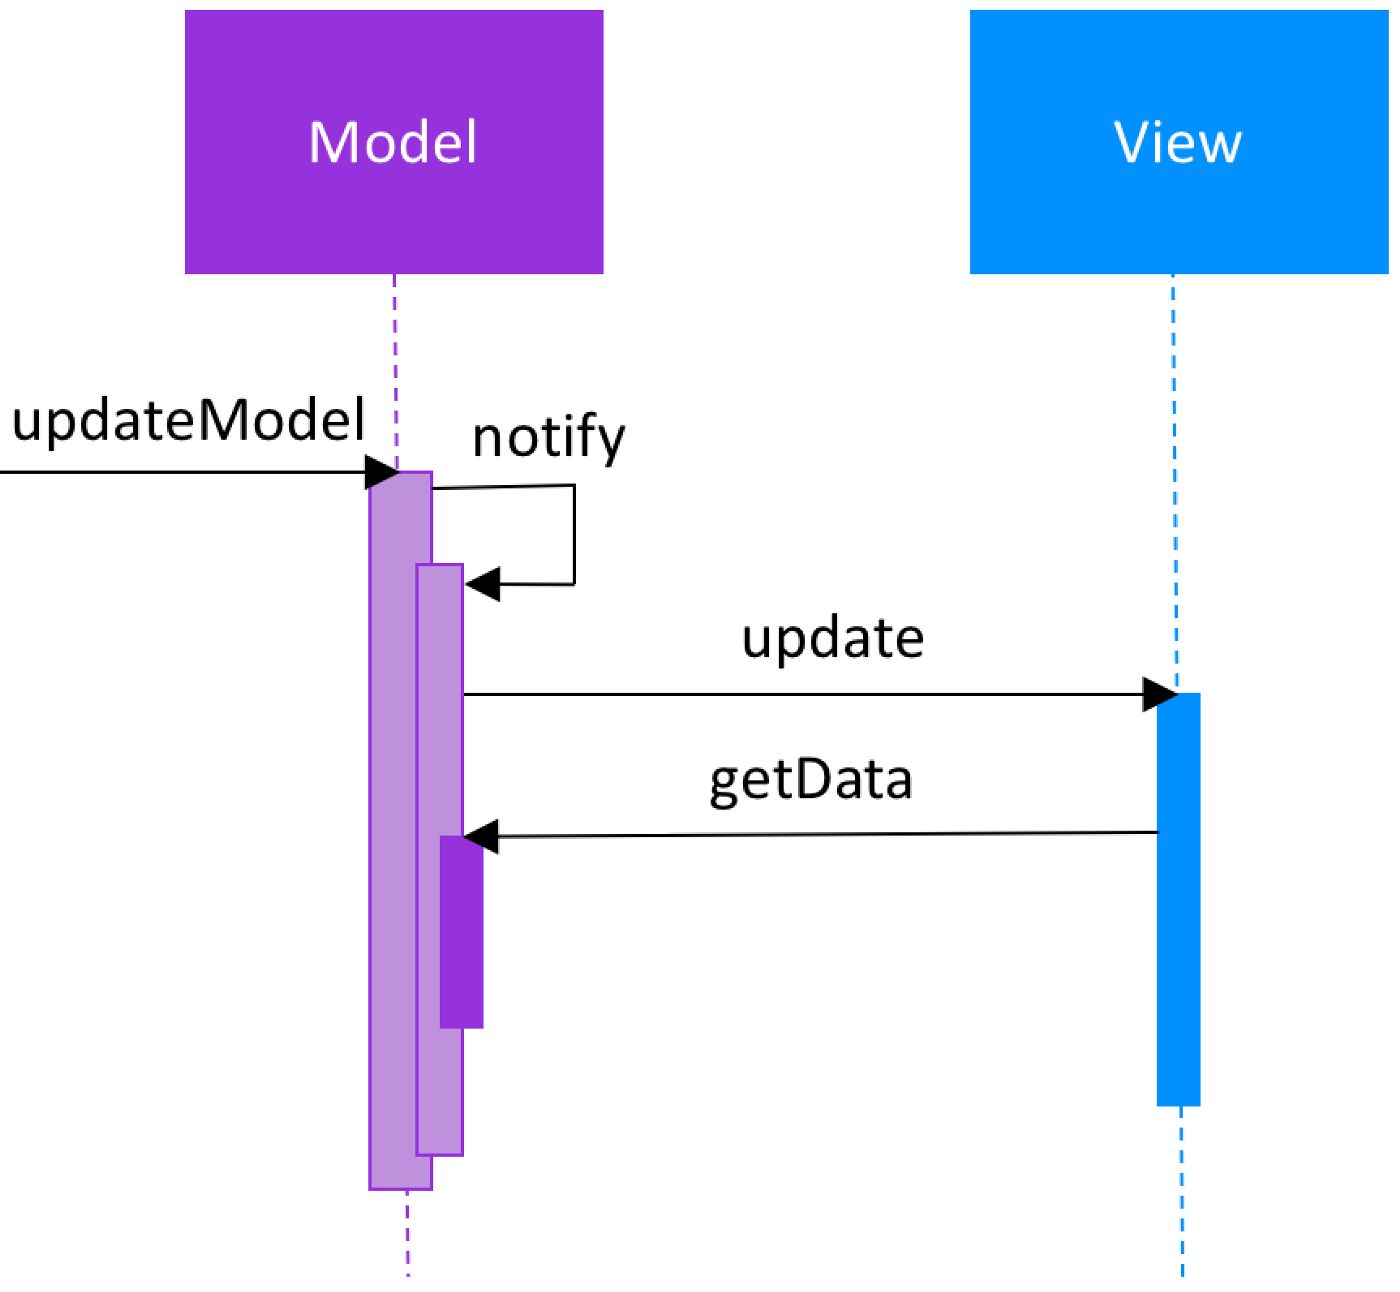
\includegraphics[width=\textwidth,height=0.8\textwidth]{image/5.png}
		\caption{Model-View-Controller — active Model — behavior}
	\end{figure}
	\subsection{应用}
	 The Activities, Fragments and Views should be the Views in the MVC world. The Controllers should be separate classes that don’t extend or use any Android class, and same for the Models.
	 \par 将Controller连接到View时会出现一个问题,因为Controller需要告知View更新。在被动Model MVC架构中,Controller需要保留对View的引用。在专注于测试的同时,最简单的方法是拥有一个BaseView接口,该接口可以扩展Activity / Fragment / View。因此,控制器将具有对BaseView的引用。
	 \par\noindent\textbf{优点:}
	 \par Model-View-Controller模式高度支持关注点分离。这一优点不仅提高了代码的可测试性,而且还使扩展变得更容易,从而可以轻松实现新功能。
	 \par Model类没有对Android类的任何引用,因此可以直接进行单元测试。 Controller不会扩展或实现任何Android类,并且应具有对View接口类的引用。这样,也可以对控制器进行单元测试。
	 \par If the Views respect \textbf{the single responsibility principle} then their role is just to update the Controller for every user event and just display data from the Model, without implementing any business logic. In this case, UI tests should be enough to cover the functionalities of the View.
	 \par\noindent\textbf{缺点:}
	 \par The View Depends On The Controller And On The Model
	 \par 为了最小化View中的逻辑,模型应该能够为要显示的每个元素提供可测试的方法。在主动的Model实现中,这将成倍增加类和方法的数量,因为需要每种类型的数据的观察者。
	 \par Given that the View depends on both the Controller and the Model, changes in the UI logic might require updates in several classes, decreasing the flexibility of the pattern.
	 \subsubsection{问题:Who Handles The UI Logic?}
	 根据MVC模式,控制器更新模型,视图从模型中获取要显示的数据。但是谁决定如何显示数据?是模型还是视图?下面是在View中展示"Lastname,Firstname"
	 \par 如果Model只提供原始数据,意味着View处理UI逻辑,这使得将会很难测试UI逻辑,code如下:
	 \begin{lstlisting}[language=Java,morekeywords={String}]
String firstName = userModel.getFirstName(); 
String lastName = userModel.getLastName(); 
nameTextView.setText(lastName + ", " + firstName)
	 \end{lstlisting}
	 \par 另一种方法是让模型仅公开需要显示的数据,从而从视图中隐藏任何业务逻辑。但是,然后,我们得到处理业务和UI逻辑的模型。它可以进行单元测试,但是模型最终隐含地依赖于View,code如下:
	 \begin{lstlisting}[language=Java,morekeywords={String}]
String name = userModel.getDisplayName(); 
nameTextView.setText(name);
	 \end{lstlisting}
	 \section{代码例子}
	 代码结构:
	 \begin{itemize}
	 	\item Bean:
	 	\subitem User: Java Bean
	 	\item Model
	 	\subitem UserModel: Model接口,提供给Controller使用
	 	\subitem UserModelImpl: Model实现,业务逻辑实现,Http请求和数据库交互
	 	\item MainActivity: 实际的Controller层,View层是xml文件,处理用户行为
	 	\item MyObserver: MainActivity的接口(实际为View接口),提供给Model层实现观察者模式,用来更新数据显示
	 \end{itemize}
	 \begin{figure}[!h]
	 	\centering
	 	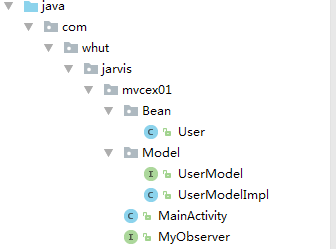
\includegraphics[width=0.6\textwidth]{image/6.png}
	 	\caption{代码目录}
	 \end{figure}
\begin{lstlisting}[language=xml]
<!--activity_main.xml-->
<LinearLayout xmlns:android="http://schemas.android.com/apk/res/android"
	android:orientation="vertical"
	android:layout_width="match_parent"
	android:layout_height="match_parent">
	<TextView
	android:id="@+id/text_username"
	android:layout_width="match_parent"
	android:layout_height="wrap_content"
	android:text="点击按钮获取用户名"
	android:textColor="#000"
	android:textSize="30sp"
	android:gravity="center_horizontal"/>
	<Button
	android:id="@+id/btn_getusername"
	android:layout_width="wrap_content"
	android:layout_height="wrap_content"
	android:layout_gravity="center_horizontal"
	android:text="获取"/>
</LinearLayout>
\end{lstlisting}
 	\begin{lstlisting}[language=java]
//Bean.User
public class User {
	private String firstname;
	private String lastname;
	//构造器, setter and getter
}
 	\end{lstlisting}
 	\begin{lstlisting}[language=java]
//Model.UserModel
public interface UserModel {
	void getDisplayName(String userid, MyObserver myObserver);
}

//Model.UserModelImpl
public class UserModelImpl implements UserModel {

	private User user;
	private final String baseurl = "http://yourbaseurl";
	
	public UserModelImpl() {
		user = new User();
	}

	@Override
	public void getDisplayName(String userid, final MyObserver myObserver) {
		OkHttpClient client = new OkHttpClient();
		final Request request = new Request.Builder().url(baseurl).method("GET",null).build();
		Call call = client.newCall(request);
		call.enqueue(new Callback() {
		@Override
		public void onFailure(Call call, IOException e) {
			myObserver.onError();
		}

		@Override
		public void onResponse(Call call, Response response) throws IOException {
			String displayname = response.body().string();
			//在Ui线程更新,这里简写
			myObserver.onSuccess(displayname);
		}
		});
	}
}
 	\end{lstlisting}
	\begin{lstlisting}[language=java]
//MyObserver
public interface MyObserver {
	void onSuccess(String displayname);
	void onError();
}

//MainActivity
public class MainActivity extends AppCompatActivity implements MyObserver {

	private Button btn;
	private TextView textView;
	
	private UserModel userModel;
	
	@Override
	protected void onCreate(Bundle savedInstanceState) {
		super.onCreate(savedInstanceState);
		setContentView(R.layout.activity_main);
		
		btn = findViewById(R.id.btn_getusername);
		textView = findViewById(R.id.text_username);
		
		userModel = new UserModelImpl();
		
		btn.setOnClickListener(new View.OnClickListener() {
			@Override
			public void onClick(View v) {
				String userid = "yourid";
				userModel.getDisplayName(userid, MainActivity.this);
			}
		});
	}
	
	private void setView(String displayname){
		textView.setText(displayname);
	}
	
	@Override
	public void onSuccess(String displayname) {
		setView(displayname);
	}
	
	@Override
	public void onError() {
		setView("获取信息失败!");
	}
}
 	\end{lstlisting}
\end{document}
